\section{Vorwort}

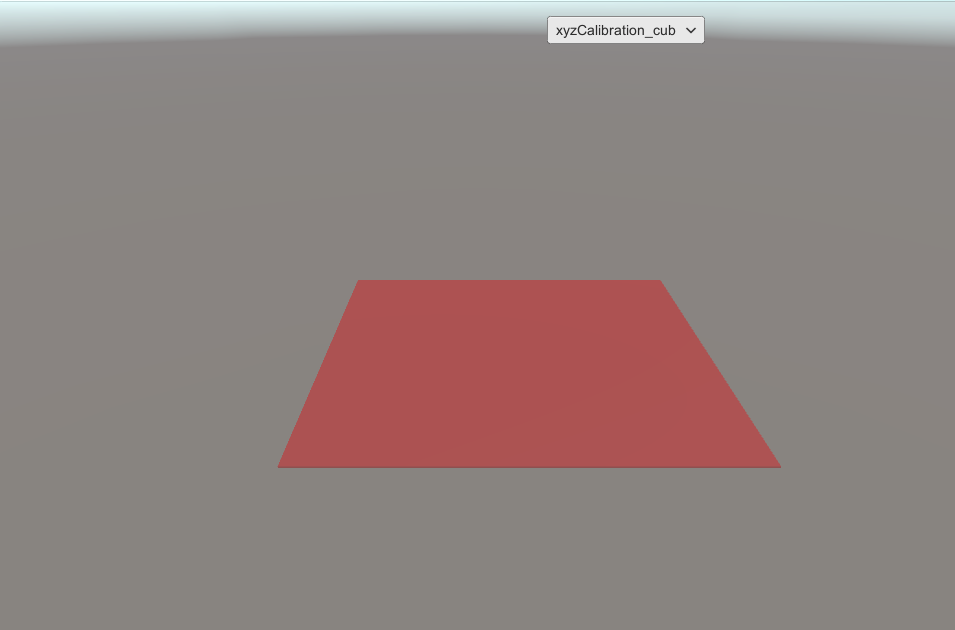
\includegraphics[width=\paperwidth-3cm]{./pictures/dropdown.png}


\section{.gcode Parser}


\monocodebox{sh}{Slicersetting Ideamaker:}{./codesnippets/xyzCalibration_cube.gcode
}{false}{0}{12}

Zur Anzeige benötigte Werte:
\begin{itemize}
  \item Dimension (Breite, Tiefe, Höhe, Düsendurchmesser)
  \item Filament Diameter
  \item Plate Shape (Rechteckig / Rund)
\end{itemize}

\monocodebox{sh}{Druck Startcode}{./codesnippets/xyzCalibration_cube.gcode
}{false}{13}{27}

Hier werden vereinfacht nur die Temperaturen gesetzt und mit \textbf{G28}die Home Position angefahren.

\newpage

\monocodebox{sh}{Druck Startcode Nozzle Prime}{./codesnippets/xyzCalibration_cube.gcode
}{false}{26}{35}

Hier wird außerhalb des Druckbereiches Material in die Düse gedrückt.
Dies ist nötig damit dann beim drucken des Models schon Material am Ausgang der Düse ist.

\monocodebox{sh}{Extruder-Mode}{./codesnippets/xyzCalibration_cube.gcode
}{false}{36}{36}

Diese Zeile ist wichtig da sie festlegt wie die nachfolgenden G codes interpretiert werden sollen.
% \monocodebox{sh}{Speedtest mittels Terminal:}{./codesnippets/speedtest.sh}{false}{0}{9999999}

% \includegraphics[scale=0.5]{./pictures/streamingarten.png}




%
% \begin{tabular}{ll}
% \centering
% \glqq Text\grqq{} und \flqq Text\frqq  & \verb+ \glqq Text\grqq{} und \flqq Text\frqq+\\
% \glq Text\grq{} und \flq Text\frq  & \verb+ \glq Text\grq{} und \flq Text\frq+
% \end{tabular}





% \definecolor{fulda_green}{rgb}{.38,.74,.10}
% \definecolor{fulda_lightgreen}{rgb}{.64,.85,.40}
% \definecolor{fulda_lightgray}{gray}{.4}
% \definecolor{fulda_subtitle}{rgb}{.38,.74,.10}
% \definecolor{fulda_title}{gray}{.0}
% \definecolor{fulda_chapter}{rgb}{.38,.74,.10}
% \definecolor{fulda_section}{rgb}{.38,.74,.10}
% \definecolor{fulda_subsection}{gray}{.4}
% \definecolor{fulda_part}{gray}{1}
% \definecolor{fulda_partnumber}{rgb}{.79,1,.55}
% \definecolor{fulda_partback}{rgb}{.64,.85,.40}
% \definecolor{fulda_highlighttitle}{rgb}{.38,.74,.10}
% \definecolor{fulda_highlightbody}{rgb}{.79,1,.55}
% \definecolor{fulda_highlighttitletext}{gray}{1}
% \definecolor{lightgray}{rgb}{0.93,0.95,1.0}
% \definecolor{darkgreen}{RGB}{82,130,179}
